\iffalse
\def\mytitle{LINE USING PYTHON}
\def\myauthor{Mukesh Guptha.CH}
\def\contact{mukeshchinta1313@gmail.com}
\def\mymodule{Future Wireless Communication (FWC)}
\documentclass[10pt, a4paper]{article}
\usepackage[a4paper,outer=1.5cm,inner=1.5cm,top=1.75cm,bottom=1.5cm]{geometry}
\twocolumn
\usepackage{graphicx}
\graphicspath{{./images/}}
\usepackage[colorlinks,linkcolor={black},citecolor={blue!80!black},urlcolor={blue!80!black}]{hyperref}
\usepackage[parfill]{parskip}
\usepackage{lmodern}
\usepackage{tikz}
	\usepackage{physics}
%\documentclass[tikz, border=2mm]{standalone}
\usepackage{karnaugh-map}
%\documentclass{article}
\usepackage{tabularx}
\usepackage{circuitikz}
\usetikzlibrary{calc}
\usepackage{amsmath}
\usepackage{amssymb}
\renewcommand*\familydefault{\sfdefault}
\usepackage{watermark}
\usepackage{lipsum}
\usepackage{xcolor}
\usepackage{listings}
\usepackage{float}
\usepackage{titlesec}
\providecommand{\mtx}[1]{\mathbf{#1}}
\titlespacing{\subsection}{1pt}{\parskip}{3pt}
\titlespacing{\subsubsection}{0pt}{\parskip}{-\parskip}
\titlespacing{\paragraph}{0pt}{\parskip}{\parskip}
\newcommand{\figuremacro}[5]{
    \begin{figure}[#1]
        \centering
        \includegraphics[width=#5\columnwidth]{#2}
        \caption[#3]{\textbf{#3}#4}
        \label{fig:#2}
    \end{figure}
}
\newcommand{\myvec}[1]{\ensuremath{\myvec{#1}}}
\let\vec\mathbf
\lstset{
frame=single, 
breaklines=true,
columns=fullflexible
}

\title{\mytitle}
\author{\myauthor\hspace{1em}\\\contact\\FWC22069\hspace{6.5em}IITH\hspace{0.5em}\mymodule\hspace{6em}ASSIGN-4}
\date{}
\begin{document}
	\maketitle
 \paragraph*{\large Problem Statement}
$-$ \textbf{
 \fi
	Find the equation of the line passing through  (-3,5) and perpendicular to the line through the points (2,5) and (-3,6).
	\begin{figure}[!ht]
		\centering
 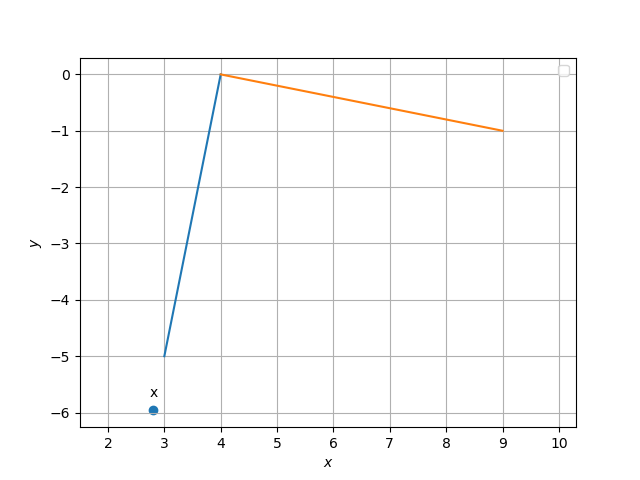
\includegraphics[width=\columnwidth]{chapters/11/10/2/10/figs/Figure_1.png}
		\caption{}
		\label{fig:11/10/2/10}
  	\end{figure}
	\\
	\solution 
	\iffalse
}
 
\begin{figure}[h]
\centering
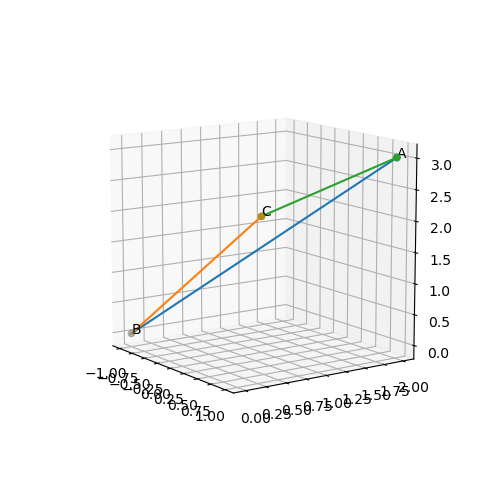
\includegraphics[width=1\columnwidth]{Figure_1.png}
\caption{perpendicular intersection}
\end{figure}
	\section*{Construction}
\vspace{2mm}
 the input parameters are as follows
{
\setlength\extrarowheight{4pt}
 
 \begin{tabular}{|c|c|c|}
	\hline
	\textbf{Symbol}&\textbf{Value}&\textbf{Description}\\
	\hline
 c&$
	\myvec{
		5\\
		-1\\
	}$
	&coefficients of line \\
	\hline
 d&$
	\myvec{
		20\\
	}$
	&constants\\
	\hline
 \end{tabular}
}
\section*{\large solution}

\subsection*{\large part 1}
\fi
Let 
\begin{align}
	\vec{A}=\myvec{2 \\5}, \vec{B}= \myvec{-3 \\ 6}, \vec{P} =\myvec{-3 \\5}
\end{align}
The normal vector of the desired  line is then given by 
\begin{align}
\vec{n} = \vec{B}-\vec{A}
=\myvec{
    5\\
    -1
}
\end{align}
Thus, the equation of the line is 
\begin{align}
\myvec{
    5 &-1
	}\brak{\vec{x} - \myvec{-3 \\5}}
= 0
\\
\implies 
\myvec{
    5 &-1
	}\vec{x} 
= -20
\end{align}
\iffalse
\begin{align}
 \myvec{
    5 & -1\\
}\myvec{
    x+3\\
    y-5\\
}
\label{eq-4}
\end{align}
The required line equation is 
\begin{align}
 5\vec{x}-\vec{y}+20=0
\label{eq-5}
\end{align}
\end{document}
\fi
